\documentclass[11pt]{article}
% Packages not pre-loaded by mdpi.cls
\usepackage{mathtools}
\usepackage[section]{placeins}
\usepackage{xurl}
\renewcommand{\ttdefault}{lmtt} % Latin Modern Typewriter (Type 1, avoids bitmap ectt)
\renewcommand\linenumberfont{\normalfont\scriptsize\fontfamily{lmss}\selectfont} % Type 1 sans for line numbers

\graphicspath{{../../figures/paper/}{figures/}}
\usetikzlibrary{arrows.meta,positioning,fit,calc}

% Lowercase aliases for MDPI's capitalized theorem environments
% (mdpi.cls defines \begin{Theorem}, our sections use \begin{theorem})
\newenvironment{theorem}{\begin{Theorem}}{\end{Theorem}}
\newenvironment{lemma}{\begin{Lemma}}{\end{Lemma}}
\newenvironment{definition}{\begin{Definition}}{\end{Definition}}
\newenvironment{corollary}{\begin{Corollary}}{\end{Corollary}}
\newenvironment{remark}{\begin{Remark}}{\end{Remark}}
\newenvironment{proposition}{\begin{Proposition}}{\end{Proposition}}
\newenvironment{example}{\begin{Example}}{\end{Example}}

% Custom commands
\newcommand{\SBT}{\textsc{SBT}}
\newcommand{\Pone}{\textbf{P1}}
\newcommand{\Ptwo}{\textbf{P2}}
\newcommand{\Pthree}{\textbf{P3}}
\newcommand{\Pfour}{\textbf{P4}}
\newcommand{\Pfive}{\textbf{P5}}
\newcommand{\Psix}{\textbf{P6}}

% Notation
\newcommand{\RM}{\mathrm{RM}}
\newcommand{\Def}{\mathrm{Def}}
\newcommand{\Lip}{\mathrm{Lip}}
\newcommand{\leanname}[1]{\path{#1}}


\title{To Count a Stone with Six Birds: A Mathematics is A Theory}
\author{Ioannis Tsiokos\textsuperscript{1}\\[2pt]
  \small\href{mailto:ioannis@automorph.io}{ioannis@automorph.io}}
\date{Version 3: 4 October 2026 \quad (Version 1: 28 January 2026)}

\newcommand{\printaffiliation}{%
  \begin{center}
    \small \textsuperscript{1}Automorph Inc., 1207 Delaware Ave \#4131, Wilmington, DE 19806, USA
  \end{center}
}

\begin{document}
\maketitle
\printaffiliation
\thispagestyle{firstpage}

% Auto-generated by scripts/export_results_tex.py from notes/math_review/
\newcommand{\StencilBaselineTotal}{\ensuremath{1000}}
\newcommand{\StencilBaselineSurvivors}{\ensuremath{913}}
\newcommand{\StencilBaselineOrderZero}{\ensuremath{913}}
\newcommand{\StencilLegacyTested}{\ensuremath{503}}
\newcommand{\StencilLegacySurvivors}{\ensuremath{50}}
\newcommand{\StencilLegacyTestedOrderOne}{\ensuremath{503}}
\newcommand{\StencilLegacyStabilityOnly}{\ensuremath{50}}
\newcommand{\StencilMatchedTotal}{\ensuremath{300}}
\newcommand{\StencilMatchedPerOrder}{\ensuremath{100}}
\newcommand{\StencilMatchedM}{\ensuremath{3}}
\newcommand{\StencilMatchedNZero}{\ensuremath{64}}
\newcommand{\StencilMatchedDTwoMax}{\ensuremath{0.050}}
\newcommand{\StencilMatchedRatioMax}{\ensuremath{0.85}}
\newcommand{\StencilMatchedStableZero}{\ensuremath{100}}
\newcommand{\StencilMatchedLeibnizZero}{\ensuremath{0}}
\newcommand{\StencilMatchedStableOne}{\ensuremath{100}}
\newcommand{\StencilMatchedLeibnizOne}{\ensuremath{100}}
\newcommand{\StencilMatchedStableTwo}{\ensuremath{81}}
\newcommand{\StencilMatchedLeibnizTwo}{\ensuremath{0}}
\newcommand{\StencilMatchedStableTotal}{\ensuremath{281}}
\newcommand{\StencilMatchedLeibnizTotal}{\ensuremath{100}}
\newcommand{\StencilHuntTested}{\ensuremath{20000}}
\newcommand{\StencilHuntPerMode}{\ensuremath{10000}}
\newcommand{\StencilHuntPassed}{\ensuremath{6}}
\newcommand{\StencilHuntFalsePositives}{\ensuremath{0}}
\newcommand{\StencilHuntMinF}{\ensuremath{0.35}}
\newcommand{\StencilMatchedLabelAgreement}{\ensuremath{300}}
\newcommand{\HolonomyEps}{\ensuremath{0.050}}
\newcommand{\HolonomyNList}{\ensuremath{\{64,128,256,512\}}}
\newcommand{\HolonomyExponent}{\ensuremath{1.46}}
\newcommand{\HolonomyFitRtwo}{\ensuremath{0.988}}
\newcommand{\HolonomyNullRMMax}{\ensuremath{0}}
\newcommand{\HolonomyRMFinest}{\ensuremath{2.25\times 10^{-4}}}
\newcommand{\IntegrationNList}{\ensuremath{\{128,256,512,1024\}}}
\newcommand{\IntegrationRMAtSmallestH}{\ensuremath{1.77\times 10^{-3}}}
\newcommand{\IntegrationRMExponent}{\ensuremath{1.000}}
\newcommand{\IntegrationFTExponent}{\ensuremath{0.5000}}
\newcommand{\IntegrationLeftTruthFinest}{\ensuremath{4.25\times 10^{-4}}}
\newcommand{\IntegrationTrapTruthFinest}{\ensuremath{6.12\times 10^{-7}}}
\newcommand{\IntegrationFTLeftMax}{\ensuremath{1.3\times 10^{-12}}}
\newcommand{\IntegrationAddMax}{\ensuremath{1.1\times 10^{-15}}}
\newcommand{\PrimeDPS}{\ensuremath{50}}
\newcommand{\PrimeNList}{\ensuremath{\{50,100,200,400,800\}}}
\newcommand{\PrimeSigmaConvList}{\ensuremath{\{1.25,1.5\}}}
\newcommand{\PrimeSigmaStripList}{\ensuremath{\{0.75,0.5\}}}
\newcommand{\PrimeTList}{\ensuremath{\{0,2,4,6\}}}
\newcommand{\PrimeRMConvAtEightHundred}{\ensuremath{0.0524}}
\newcommand{\PrimeRMStripAtEightHundred}{\ensuremath{5.01\times 10^{12}}}
\newcommand{\PrimeRMStripAtFifty}{\ensuremath{340}}
\newcommand{\PrimeErrPStripAtEightHundred}{\ensuremath{2.17\times 10^{14}}}
\newcommand{\PrimeErrSStripAtEightHundred}{\ensuremath{43.7}}
\newcommand{\PrimeCheckDPS}{\ensuremath{80}}
\newcommand{\PassivityN}{\ensuremath{12}}
\newcommand{\PassivityBeta}{\ensuremath{0.7}}
\newcommand{\PassivityJScale}{\ensuremath{0.5}}
\newcommand{\PassivityMeanDevLamOne}{\ensuremath{0.872}}
\newcommand{\PassivityMaxDevLamOne}{\ensuremath{7.11}}
\newcommand{\PassivityMeanDevLamZero}{\ensuremath{1.6\times 10^{-15}}}
\newcommand{\PassivityMaxDevLamZero}{\ensuremath{6.0\times 10^{-15}}}
\newcommand{\PassivityComponentsLamZero}{\ensuremath{3,3,4,1,1}}
\newcommand{\PassivityCheckDPS}{\ensuremath{80}}
\newcommand{\PassivityMatchLamOne}{\ensuremath{4.9\times 10^{-12}}}
\newcommand{\PassivityMatchLamZero}{\ensuremath{6.0\times 10^{-15}}}
\newcommand{\LeanExportCount}{\ensuremath{17}}
\newcommand{\PythonTestsPassed}{\ensuremath{18}}


\begin{abstract}
Limits, completions, and analytic continuations are usually introduced as definitions. This paper asks an operational question instead: when does a large discrete protocol, such as a difference quotient, a cumulative sum, or a truncated Euler product, admit a stable continuous closure, and how can that be tested without overclaiming? We instantiate the Six Birds framework as a closure-and-audit method for mathematics. A discrete object is staged by refinement, the cost of compressing it is tracked by an explicit defect ledger, and a packaged object is accepted only when the ledger is controlled under refinement and the relevant operations descend to the packaged layer. The formal core is machine-checked in Lean~4 with mathlib: the exact finite-difference product rule with its remainder term; a limit bridge showing that convergent factor quotients force the product quotient to converge to the Leibniz value; the classification of $R$-linear derivations of $R[X]$ by their value on $X$; and the two contracts that make packaging well defined, namely that vanishing distance in a pseudometric is an equivalence relation and that uniformly Lipschitz stage operators respect it. Four numerical exhibits then audit concrete closures. In a matched population of 300 candidate stencils, a stability gate alone retains identity-like, first-derivative, and second-derivative operators (100, 100, and 81 of 100 each), whereas adding a shrinking Leibniz defect retains only the 100 first-derivative stencils. Under a small change of coordinates, two routes for computing a derivative approach each other under refinement, with a fitted exponent of about 1.46 over four grids. For the zeta function, additive and multiplicative staged closures provably converge to a common limit when $\Re(s)>1$, and on the tested grid their route mismatch falls to 0.052 at cutoff 800; on a grid in the critical strip, with a symmetrized packaging map, the same naive truncations drift apart, reaching a mismatch of $5.0\times 10^{12}$ at the same cutoff. In an Ising partition polynomial, shrinking the negative couplings to zero reduces the mean distance of the zeros from the unit circle from 0.87 to rounding level, the endpoint being an instance of the Lee--Yang circle theorem. The diagnostics prove no new theorem about $\zeta$ or its zeros. Their value is a reproducible, failure-capable way to separate feasible closures from artifacts of the chosen protocol.
\end{abstract}

\vspace{1ex}
\noindent\textbf{Keywords:} emergence calculus; closure; audit; refinement; route mismatch; finite differences; derivations; lean

\section{Introduction}
\label{sec:introduction}

\subsection{From counting to closure}
The oldest way to count a stone is to repeat one small action many times: a tick mark, a step along a line, one more unit added to a running total.
Calculus replaces such long chains of small actions with a compressed law.
A difference quotient taken over ever finer steps becomes a derivative; a cumulative sum over ever finer cells becomes an integral.
The replacement is so familiar that it is easy to forget it is a choice, and that the choice can fail.

This paper treats that replacement as a \emph{closure problem}.
The question is not how derivatives or integrals are defined, but which compressions of a discrete protocol remain coherent as the protocol is refined, and how one can check this coherence with tests that are able to fail.
The same question arises whenever a large discrete structure is compressed into a continuous or spectral object: the primes into the zeta function, a finite spin system into the zeros of its partition polynomial, a family of local charts into a global derivative.

We answer it with the vocabulary of the Six Birds framework \cite{SixBirdsFramework}.
In that vocabulary, refinement is \emph{staging} (\Pfour), the bookkeeping of what a compression loses is \emph{accounting} (\Psix), the limit object is a \emph{package} (\Pfive), coherence requirements on the package are \emph{constraints} (\Ptwo), the rescaling or rewriting needed to make a discrete operation survive the limit is an \emph{operator rewrite} (\Pone), and the disagreement between two reasonable routes to the same object is a \emph{protocol} or holonomy defect (\Pthree).
Section~\ref{sec:dictionary} makes this dictionary precise; nothing in the mathematics depends on the names.

\subsection{Scope}
The paper is a worked instantiation of the framework in mathematics.
It translates the six roles into standard notions---limits, quotients, completions, rescalings, compatibility conditions---and it backs each claim either by a short proof, by a machine-checked Lean statement, or by a numerical diagnostic whose outcome was not fixed in advance.
It proposes no new foundations or axioms, and it does not claim that one mechanism accounts for all of mathematics.
The numerical exhibits on primes and on zeros of polynomials prove nothing about the Riemann zeta function or its zeros; they are controlled experiments that show how a closure claim can be audited.
When a diagnostic fails, as it does on the critical-strip grid, the failure is reported as information about a missing feasibility condition.

\subsection{Results}
The paper makes two kinds of contribution.

\paragraph{Formal anchors.}
Except where noted, the statements below are proved in Lean~4 with mathlib \cite{moura2021lean4,mathlib2020lean}, and none uses an axiom beyond the three standard ones of Lean's classical logic (Appendix~\ref{app:formal}).
\begin{itemize}
  \item The scaled forward difference satisfies an exact product rule with an explicit remainder, $\delta_h(fg)=(\delta_h f)g+f(\delta_h g)+h\,\delta_h f\,\delta_h g$, over any field and any nonzero step (Lemma~\ref{lem:finite-diff-leibniz}).
  \item If the factor quotients converge along a sequence (or filter) of steps tending to zero, the product quotient converges, and its limit is the Leibniz value (Proposition~\ref{prop:limit-bridge}). Bounded factor quotients alone do not suffice (Example~\ref{ex:bounded-not-convergent}). What boundedness \emph{does} buy is a derivation with values in a quotient of bounded sequences (Proposition~\ref{prop:quotient-derivation}, proved in the text).
  \item Over any commutative semiring $R$, an $R$-derivation of $R[X]$ (one that is $R$-linear and kills the coefficients) is determined by its value on $X$, and the derivation with $D(X)=p$ is $q\mapsto p\,q'$ (Theorem~\ref{thm:derivation-determined-by-X}).
  \item Packaging ``up to vanishing defect'' is a well-defined equivalence when the defect is a pseudometric (Proposition~\ref{prop:packaging}), and a family of stage operators respects it when the operators are uniformly Lipschitz (Proposition~\ref{prop:descent}). For continuous linear maps, the gain of a direct route is at most the product of the gains along a composite route plus their operator-norm route defect (Proposition~\ref{prop:route-gain}).
\end{itemize}

\paragraph{Numerical exhibits.}
Each exhibit stages a discrete protocol, records a defect ledger, and asks whether the ledger is controlled under refinement.
\begin{itemize}
  \item \emph{Calculus (Section~\ref{sec:exhibit-calculus}).} In a matched population of candidate stencils, a refinement-stability gate keeps identity-like, first-derivative, and second-derivative operators alike; adding a shrinking Leibniz defect keeps only the first-derivative ones. Cumulative sums behave as integrals: two quadrature routes converge to each other and to the exact antiderivative at their classical rates.
  \item \emph{Coordinate change (Section~\ref{sec:exhibit-holonomy}).} Two routes for computing a derivative after a change of variables disagree at finite resolution and approach each other under refinement.
  \item \emph{Primes (Section~\ref{sec:exhibit-prime}).} Additive (Dirichlet) and multiplicative (Euler) staged closures of $\zeta$ converge to a common limit for $\Re(s)>1$, by a short proof, and their mismatch decreases on the tested grid and cutoffs. On a tested grid in the critical strip, with a different (symmetrized) packaging map, the same naive truncations drift apart as the cutoff grows.
  \item \emph{Positivity (Section~\ref{sec:exhibit-passivity}).} In an Ising partition polynomial, removing negative couplings moves the zeros onto the unit circle; the endpoint is an instance of the Lee--Yang theorem \cite{LeeYang1952}.
\end{itemize}

Every number in the tables, the figures, and the generated macros of the text is produced by scripts from commit-visible artifacts in the companion repository (Section~\ref{sec:reproducibility}), which is available at \url{https://github.com/ioannist/six-birds-mathematics}.

\subsection{Organization}
Section~\ref{sec:dictionary} sets out the dictionary between the six roles and mathematical practice.
Section~\ref{sec:packaging-engine} turns it into a ``closure engine'' with explicit contracts for packaging and descent.
Sections~\ref{sec:exhibit-calculus}--\ref{sec:exhibit-passivity} present the four exhibits.
Section~\ref{sec:reproducibility} describes how the results are regenerated, and Section~\ref{sec:discussion} discusses scope and next steps.
Appendix~\ref{app:formal} lists the Lean declarations, and Appendix~\ref{app:versions} records the version history.

\section{The Six Birds dictionary for mathematical closures}
\label{sec:dictionary}

The Six Birds framework \cite{SixBirdsFramework} names six roles that recur whenever a detailed description is compressed into a coarser one that is still supposed to obey laws.
In this paper the roles are a naming convention: each one marks a piece of data that must be supplied explicitly when a discrete protocol is compressed into a stable mathematical object.
The dictionary is adopted, not derived.
For every exhibit we supply the carrier, the comparison, the packaging, and the audit by hand; none of them follows from the six labels, and the framework's own structural hypotheses (such as its bounded-interface assumption) are not tested by the experiments here.

\subsection{The six roles}
In mathematics the objects playing these roles are usually families indexed by a refinement parameter (meshes, truncations, partitions), error terms and residual norms, quotient or completion maps, and coherence conditions such as linearity, locality, invariance, or compatibility with products.

\begin{remark}[The six roles in mathematical form]\label{rem:six-primitives}
Let $\mathcal P$ be a set of protocol objects (discrete descriptions), refined along a stage parameter $j$ (or a step size $h\downarrow 0$).
\begin{enumerate}
  \item \Pfive\ (Packaging). An equivalence relation $\sim$ on $\mathcal P$ identifies descriptions that should count as the same object, with quotient map $\Pi:\mathcal P\to\mathcal P/\!\sim$.
  The map $\Pi$ changes type, so it is not itself an idempotent endomap.
  The idempotent object is the \emph{saturation} of sets of descriptions,
  \[
    \mathrm{cl}(A)\;:=\;\Pi^{-1}\bigl(\Pi(A)\bigr),\qquad A\subseteq\mathcal P,
  \]
  which is extensive, monotone, and idempotent, that is, a closure operator \cite{DaveyPriestley2002}.
  A finer equivalence identifies less, so its saturation is smaller and has more fixed points.
  In analytic instances, $\sim$ is ``equal up to a defect that vanishes under refinement'' (Section~\ref{subsec:packaging}); in algebraic instances it is a congruence.

  \item \Psix\ (Accounting). A ledger is a designated family of nonnegative diagnostics: error bounds, residual norms, route-mismatch statistics.
  In this paper the ledger records feasibility, that is, whether the compression stays coherent under refinement; it is not an arrow-of-time certificate.
  Refinement orders can support monotone information measures, but they do not by themselves make an approximation error decrease. Whether the ledger shrinks is something we test, never something we assume.

  \item \Pfour\ (Staging). The refinement parameter $j$ or $h$ is the stage. Staging is nontrivial when refinement genuinely increases resolution rather than merely reparametrizing.

  \item \Ptwo\ (Constraints). Coherence conditions imposed on the packaged layer: linearity, a product rule, an invariance, or compatibility with an algebraic operation.

  \item \Pone\ (Operator rewrite). A micro-operator $F:\mathcal P\to\mathcal P$ induces a packaged operator $F^\sharp([p]):=[F(p)]$ exactly when
  \[
    p\sim q\ \Longrightarrow\ F(p)\sim F(q).
  \]
  When this fails, one must change the comparison, rescale or otherwise rewrite $F$ (for example by the factor $h^{-1}$ that turns a difference into a difference quotient), or accept that no packaged operator exists.

  \item \Pthree\ (Protocol). When two admissible routes produce objects of the same type (``refine, then apply'' versus ``apply, then refine''), their discrepancy is a route-mismatch defect $\RM$. In stable regimes it should shrink under refinement.
\end{enumerate}
\end{remark}

\subsection{``A mathematics is A theory''}
The framework organizes an instantiation as a \emph{theory package}: a carrier, a lens, a completion rule, and an audit \cite{SixBirdsFramework}.
We keep the same shape and read the audit as a defect ledger.

\begin{definition}[Mathematics theory package]\label{def:math-theory-package}
A \emph{mathematics theory package} is a tuple $\mathcal T=(Z,\ f,\ \Sigma_f,\ E,\ \mathcal D)$ where
\begin{itemize}
  \item $Z$ is a carrier of discrete protocol objects at a chosen stage (grid functions, truncated sums or products, finite compositions, sequences of rationals);
  \item $f:Z\to X$ is a \emph{lens}, a coarse description map, and $\Sigma_f$ is the family of predicates on $Z$ that are visible through $f$, that is, constant on the fibers of $f$;
  \item $E:\mathcal V\to\mathcal V$ is a \emph{completion} or packaging endomap on a description space $\mathcal V$ associated with $Z$, idempotent or approximately idempotent in a stated norm, whose fixed points are the objects the package treats as complete;
  \item $\mathcal D$ is a \emph{defect ledger}, a designated family of nonnegative diagnostics together with the behaviour required of them under refinement (typically, decay to zero along the stage parameter). That behaviour is stated as a hypothesis or tested; it is not built into the definition.
\end{itemize}
\end{definition}

\begin{remark}[The title phrase]\label{rem:math-is-theory}
``A mathematics is A theory'' is meant in the following sense.
To introduce a stable mathematical layer is to specify (i) which discrete protocol objects are staged, (ii) which identifications are permitted under refinement, (iii) which completion or packaging map is used, and (iv) which defect ledger certifies that the packaged layer is coherent.
\end{remark}

\subsection{Notation}
We write $h>0$ for a step size and $h\downarrow 0$ for refinement; equivalently, a depth index $j\to\infty$.
Families of discrete objects carry stage subscripts ($A_h$, $F_h$, $z_h$).
Throughout, a route mismatch compares two routes $R_1(h)$ and $R_2(h)$ that produce outputs on a common comparison space:
\begin{equation}\label{eq:rm-generic}
  \RM(h)\;=\;\frac{\|R_1(h)-R_2(h)\|}{\|R_1(h)\|+\varepsilon_0},
\end{equation}
where $\varepsilon_0>0$ is a small constant that only guards against division by zero.
This is a \emph{relative} diagnostic.
Section~\ref{sec:exhibit-holonomy} instantiates it for a change of coordinates, Section~\ref{sec:exhibit-calculus} for two quadrature rules, and Section~\ref{sec:exhibit-prime} for two staged descriptions of~$\zeta$.

\section{A closure engine for mathematics}
\label{sec:packaging-engine}

This section states the procedure that the exhibits apply.
It does not re-found analysis; it makes explicit the commitments that are usually left tacit when one passes from a discrete protocol to a packaged law.
There are five of them---staging, a ledger, a packaging contract, a descent contract, and route diagnostics---and Figure~\ref{fig:engine} shows how they fit together.

\begin{figure}[htbp]
\centering
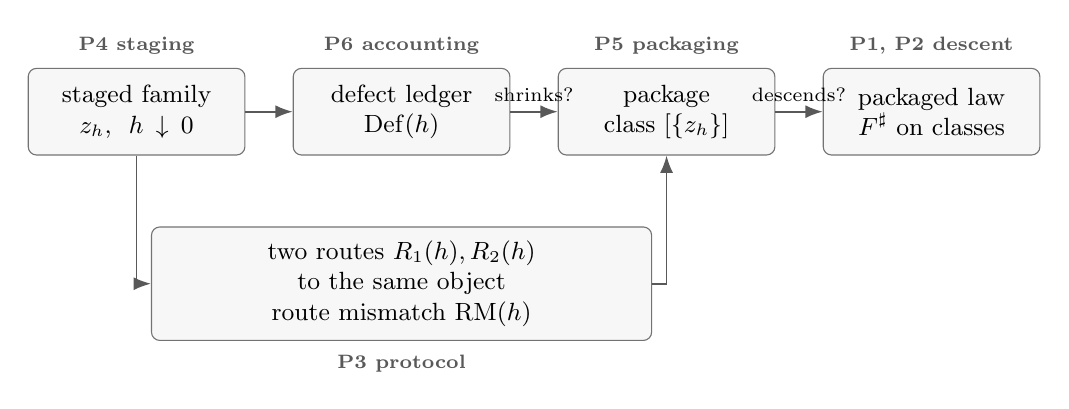
\begin{tikzpicture}[
  font=\small,
  box/.style={draw=black!55, rounded corners=3pt, fill=black!3, align=center, inner sep=5pt, minimum height=11mm, text width=24mm},
  arr/.style={-{Latex[length=2.2mm]}, draw=black!65, line width=0.6pt},
  tag/.style={font=\scriptsize\bfseries, text=black!65}
]
\node[box] (stage) {staged family\\ $z_h$, \ $h\downarrow 0$};
\node[box, right=6mm of stage] (ledger) {defect ledger\\ $\Def(h)$};
\node[box, right=6mm of ledger] (pack) {package\\ class $[\{z_h\}]$};
\node[box, right=6mm of pack] (law) {packaged law\\ $F^\sharp$ on classes};
\node[box, below=9mm of ledger, text width=60mm] (routes) {two routes $R_1(h),R_2(h)$ to the same object\\ route mismatch $\RM(h)$};
\draw[arr] (stage) -- (ledger);
\draw[arr] (ledger) -- node[above, font=\scriptsize]{shrinks?} (pack);
\draw[arr] (pack) -- node[above, font=\scriptsize]{descends?} (law);
\draw[arr] (stage.south) |- (routes.west);
\draw[arr] (routes.east) -| (pack.south);
\node[tag, above=0.5mm of stage] {P4 staging};
\node[tag, above=0.5mm of ledger] {P6 accounting};
\node[tag, above=0.5mm of pack] {P5 packaging};
\node[tag, above=0.5mm of law] {P1, P2 descent};
\node[tag, below=0.5mm of routes] {P3 protocol};
\end{tikzpicture}
\caption{The closure engine. A staged family is audited by a defect ledger. If the defect vanishes under refinement in a genuine pseudometric, the family defines a packaged object (Proposition~\ref{prop:packaging}). A discrete operator becomes a packaged law only if it respects the packaging (Proposition~\ref{prop:descent}), which may require rescaling or rewriting it. Independently, two routes to the same object are compared by a route mismatch that should shrink in stable regimes.}
\label{fig:engine}
\end{figure}

\subsection{Staging (\Pfour)}
Fix a family of discrete protocol spaces $\{Z_h\}_{h>0}$ indexed by a refinement parameter: a mesh size, a truncation cutoff, a partition diameter.
A point $z_h\in Z_h$ is a description at stage $h$.
Often there are comparison maps $\rho_{h\to h'}:Z_h\to Z_{h'}$ for $h'<h$ that carry coarse objects to finer resolution (interpolation, refinement of a partition, extension of a truncation).
Staging is what turns ``infinitely many small steps'' into a question about the behaviour of a family as $h\downarrow 0$, and therefore into something that can be tested.

\subsection{Ledgers and feasibility gates (\Psix)}
A closure claim is meaningful only relative to a ledger of nonnegative diagnostics that measure what a compression loses.
We use two kinds:
\begin{enumerate}
  \item \emph{approximation errors}, comparing a candidate quantity across refinement, $\|Q_h-Q_{h'}\|$, or against a reference, $\|Q_h-Q_\star\|$;
  \item \emph{coherence defects}, measuring the failure of an intended algebraic constraint, such as a Leibniz defect for a product rule or a route mismatch between two protocols.
\end{enumerate}
A \emph{feasibility gate} is a requirement on the ledger, either asymptotic ($\Def(h)\to 0$ as $h\downarrow 0$) or, in finite experiments, a contraction test such as $\Def(h')\le\theta\,\Def(h)$ for $h'<h$ and some $\theta<1$, together with an absolute threshold.
A finite gate checks finitely many stages; it is evidence about the trend, not a proof of the limit.

\subsection{Packaging as identification (\Pfive)}
\label{subsec:packaging}
Packaging turns a staged family into an object by identifying families whose differences vanish under refinement.
This is the pattern of the Cauchy completion of the rationals and of identifying two difference quotients that differ by $o(1)$.
For it to define objects at all, the identification must be an equivalence relation, and an arbitrary nonnegative defect does not guarantee that.

\begin{example}[A defect that does not package]\label{ex:nontransitive}
On three points $a,b,c$ put $d(a,b)=d(b,c)=0$, $d(a,c)=1$, with $d$ symmetric and zero on the diagonal.
Taking $d$ independent of the stage, ``$d$ tends to zero'' relates $a$ to $b$ and $b$ to $c$ but not $a$ to $c$.
\end{example}

The missing ingredient is the triangle inequality.
We therefore make the comparison space part of the packaging contract.

\begin{proposition}[Packaging contract]\label{prop:packaging}
Let $(X,d)$ be a pseudometric space. For sequences $a,b:\mathbb N\to X$ write $a\sim b$ when $d(a_n,b_n)\to 0$. Then $\sim$ is an equivalence relation.
\end{proposition}

\begin{proof}
Reflexivity and symmetry follow from $d(x,x)=0$ and $d(x,y)=d(y,x)$. For transitivity, $0\le d(a_n,c_n)\le d(a_n,b_n)+d(b_n,c_n)\to 0$.
\end{proof}

\noindent In Lean this is \leanname{Closure.vanishingDistSetoid}.
Several ledger coordinates can be combined through a joint pseudometric or as a conjunction of such relations.
Three further points keep the contract honest.
\begin{itemize}
  \item \emph{A quotient is not a limit.} The quotient by $\sim$ of \emph{all} sequences is not a completion: bounded oscillating scalar sequences survive in $\ell^\infty/c_0$ without representing any real number. A completion requires restricting to Cauchy sequences, and convergence in an existing complete space must be proved there.
  \item \emph{Algebra need not descend.} On unbounded scalar sequences, multiplication does not respect $\sim$: $n$ and $n+1/n$ are equivalent, but their squares differ by $2+1/n^2$. On uniformly bounded families it does, by $|ab-a'b'|\le|a|\,|b-b'|+|b'|\,|a-a'|$.
  \item \emph{The stage dependence must be uniform.} A comparison that changes with the stage needs the same triangle-type control uniformly in the stage; naming a ledger does not supply it.
\end{itemize}

\subsection{Descent of operators (\Pone, \Ptwo)}
A discrete operator family $F_n$ becomes a packaged law only if equivalent inputs give equivalent outputs.
A uniform Lipschitz estimate is a sufficient condition.

\begin{proposition}[Descent contract]\label{prop:descent}
Let $X,Y$ be pseudometric spaces and $F_n:X\to Y$ maps with $d_Y(F_n x,F_n y)\le K\,d_X(x,y)$ for all $n,x,y$, where $K\ge 0$ does not depend on $n$.
If $d_X(a_n,b_n)\to 0$, then $d_Y(F_n a_n,F_n b_n)\to 0$. Hence $(a_n)\mapsto(F_n a_n)$ induces a map on equivalence classes.
\end{proposition}

\begin{proof}
$0\le d_Y(F_n a_n,F_n b_n)\le K\,d_X(a_n,b_n)\to 0$.
\end{proof}

\noindent In Lean this is \leanname{Closure.stage_operator_respects_vanishing_dist}.
The condition is sufficient, not necessary, and it genuinely fails for the operator at the heart of calculus if the comparison is chosen carelessly.

\begin{example}[Difference quotients do not descend on uniform values]\label{ex:no-descent}
Let $h_n=1/n$, $f_n(x)=h_n\sin(x/h_n)$ and $g_n=0$. Then $\|f_n-g_n\|_\infty\le h_n\to 0$, yet $\delta_{h_n}f_n(0)=\sin(1)\ne 0=\delta_{h_n}g_n(0)$.
The Lipschitz constant of $\delta_h$ with respect to the uniform norm is of order $1/h$, so Proposition~\ref{prop:descent} does not apply.
\end{example}

The repair is a richer comparison, which is an instance of \Pone.
If $f,g\in C^1$, the mean value theorem gives $\|\delta_h(f-g)\|_\infty\le\|f'-g'\|_\infty$ on any interior domain, so equivalence of inputs in the $C^1$ norm descends to equivalence of outputs in the $C^0$ norm.
For an operator that maps a function algebra to itself, one works on a derivative-closed class such as polynomials or smooth functions with derivative seminorms.

\subsection{Route mismatch (\Pthree)}
When two reasonable routes $R_1(h)$ and $R_2(h)$ produce outputs on a common space, the relative mismatch~\eqref{eq:rm-generic} is a computable defect, and its decay under refinement indicates a stable regime.
For bounded linear routes the absolute version of this defect has a clean meaning: it controls how much the direct route can amplify compared with the composite one.

\begin{proposition}[Route defect bounds gain]\label{prop:route-gain}
Let $A$, $B$, $C$ be continuous linear maps between normed spaces with $C$ and $A\circ B$ of the same type. Then
\[
  \|C\|\;\le\;\|A\|\,\|B\|+\|C-A\circ B\|.
\]
For a continuous linear endomap $L$, moreover $L\circ L-L=L\circ(L-\mathrm{Id})$, so $\|L\circ L-L\|\le\|L\|\,\|L-\mathrm{Id}\|$.
\end{proposition}

\noindent These are \leanname{Closure.route_gain_bound}, \leanname{Closure.idempotence_factorization}, and \leanname{Closure.idempotence_defect_bound}.
Linearity matters: for $E(x)=|x|$ on $\mathbb R$ one has $E\circ E-E=0$ but $E\bigl((E-\mathrm{Id})(-1)\bigr)=2$, so the factorization fails for nonlinear maps.
The bound concerns the absolute operator-norm defect.
The relative diagnostic used in the exhibits is evaluated on finitely many sampled inputs; rescaling it recovers only the absolute discrepancy on those inputs, not the operator-norm defect. (For $A=B=\mathrm{Id}$ and $C=\mathrm{diag}(1,M)$ with $M>1$ on Euclidean $\mathbb R^2$, sampling only $e_1$ shows zero mismatch although $\|C-A\circ B\|=M-1$.) Applying the gain bound therefore requires a separately established operator-norm estimate, and even a zero route defect at each step does not by itself control growth over many steps.
Above all, route mismatch is a diagnostic of closure feasibility; it does not certify a direction of time or any irreversibility.

\subsection{Closure ladders}
The engine composes.
Once a packaged layer is stable it becomes the substrate for further staging and packaging: the reals arise by completing the rationals, calculus arises by packaging difference and sum protocols under coherence constraints, and geometric obstructions appear as route dependence when local descriptions are patched together.
The exhibits that follow are small, auditable instances of this pattern.

\section{Calculus as a stable closure}
\label{sec:exhibit-calculus}

This section applies the engine to the most familiar case: how differentiation and integration arise as stable closures of discrete protocols.
It has three parts: an exact ledger for products (Sections~\ref{subsec:ledger}--\ref{subsec:poly}), a numerical test of whether that ledger selects derivative-like operators from a population of candidates (Section~\ref{subsec:stencils}), and the corresponding audit for sums (Section~\ref{subsec:integration}).

\subsection{Discrete substrate}
Fix a step $h\ne 0$ and functions on a set where translation by $h$ makes sense (a grid, a line, or a field).
The substrate provides the shift $(T_hf)(x)=f(x+h)$, the difference $\Delta_h=T_h-I$, and the scaled difference
\[
  \delta_hf(x)\;:=\;\frac{f(x+h)-f(x)}{h}.
\]
The factor $h^{-1}$ is the simplest operator rewrite (\Pone): without it, the difference of a smooth function vanishes as $h\to 0$ and nothing survives refinement.
Refinement $h\to 0$ is the staging (\Pfour).

\subsection{The ledger: an exact product rule with remainder}
\label{subsec:ledger}
At finite $h$ the scaled difference is not a derivation, but its failure is exactly computable.

\begin{lemma}[Finite-difference Leibniz identity]\label{lem:finite-diff-leibniz}
Let $F$ be a field, $h\in F$ with $h\ne 0$, and $f,g:F\to F$. For all $x\in F$,
\[
  \delta_h(fg)(x)\;=\;\delta_hf(x)\,g(x)\;+\;f(x)\,\delta_hg(x)\;+\;h\,\delta_hf(x)\,\delta_hg(x).
\]
Moreover, $\delta_h$ is linear and annihilates constants.
\end{lemma}

\begin{proof}
Expand $f(x+h)g(x+h)-f(x)g(x)=\bigl(f(x+h)-f(x)\bigr)g(x)+f(x)\bigl(g(x+h)-g(x)\bigr)+\bigl(f(x+h)-f(x)\bigr)\bigl(g(x+h)-g(x)\bigr)$ and divide by $h$.
\end{proof}

\noindent The Lean statements are \leanname{Diff.delta_mul_leibniz}, \leanname{Diff.delta_add}, \leanname{Diff.delta_const_mul}, and \leanname{Diff.delta_const}, in \path{lean/Diff/FiniteDifference.lean}.
The identity is purely algebraic; it needs neither limits nor characteristic zero.

The remainder $h\,\delta_hf\,\delta_hg$ is the ledger term (\Psix) for the passage from differences to derivatives.
It carries an explicit factor of the stage parameter, so it vanishes as $h\to 0$ whenever the two factor quotients stay bounded.
That observation is the heart of the closure story, but turning it into a theorem requires care about what ``the limit'' is.

\subsection{From a vanishing remainder to derivations}
\label{subsec:bridge}
The first route identifies the packaged operator with ordinary pointwise limits.

\begin{proposition}[Limit bridge]\label{prop:limit-bridge}
Let $l$ be a filter on an index set, and let $h_i\in\mathbb R$ with $h_i\to 0$ along $l$ and $h_i\ne 0$ eventually.
Let $f,g:\mathbb R\to\mathbb R$ and $x\in\mathbb R$, and suppose $\delta_{h_i}f(x)\to a$ and $\delta_{h_i}g(x)\to b$. Then
\[
  \delta_{h_i}(fg)(x)\;\longrightarrow\;a\,g(x)+f(x)\,b .
\]
If, in addition, $l$ is nontrivial and $\delta_{h_i}(fg)(x)\to c$, then $c=a\,g(x)+f(x)\,b$.
\end{proposition}

\begin{proof}
By Lemma~\ref{lem:finite-diff-leibniz}, eventually
\[
  \delta_{h_i}(fg)(x)=\delta_{h_i}f(x)\,g(x)+f(x)\,\delta_{h_i}g(x)+h_i\,\delta_{h_i}f(x)\,\delta_{h_i}g(x).
\]
The first two terms converge to $a\,g(x)$ and $f(x)\,b$, and the third to $0\cdot a\cdot b=0$, by continuity of addition and multiplication. Uniqueness of limits in a Hausdorff space along a nontrivial filter gives the second claim.
\end{proof}

\noindent These are \leanname{Diff.tendsto_delta_mul} and \leanname{Diff.leibniz_of_tendsto_delta}.
Two features matter.
The convergence of the product quotient is \emph{derived}, not assumed.
And the nontriviality hypothesis is needed for the identification: along the trivial filter every value is a limit.

Combined with the linearity in Lemma~\ref{lem:finite-diff-leibniz}, Proposition~\ref{prop:limit-bridge} shows that on any algebra of functions where the limits $D f(x)=\lim\delta_{h_i}f(x)$ exist, all taken along the same nontrivial filter, $D$ is linear, kills constants, and satisfies $D(fg)=(Df)g+f(Dg)$.
The values of $D$ may lie in a different regularity class from its inputs; differentiation maps $C^1$ to $C^0$, while polynomials are closed under formal differentiation.
A limit along one sequence of steps is also weaker than a derivative along all steps; the filter must be stated.

Bounded factor quotients make the ledger term vanish, but they do not make the quotients converge.

\begin{example}[A vanishing ledger without a derivative]\label{ex:bounded-not-convergent}
Let $f(0)=0$ and $f(x)=x\sin(\log|x|)$ for $x\ne 0$. Then $\delta_hf(0)=\sin(\log|h|)$ is bounded by $1$ but has no limit as $h\to 0$. With $g=f$, the ledger term $h\sin^2(\log|h|)$ tends to $0$, yet $f'(0)$ does not exist.
\end{example}

So a shrinking ledger alone does not construct a derivative.
It does, however, construct a derivation if the target is chosen to be the space where bounded families live.

\begin{proposition}[A quotient-valued derivation]\label{prop:quotient-derivation}
Let $A$ be the real algebra of bounded Lipschitz functions $\mathbb R\to\mathbb R$ and $B$ the Banach algebra of bounded functions with the uniform norm. Let
\[
  Q\;=\;\ell^\infty(\mathbb N;B)\,/\,c_0(\mathbb N;B),
\]
regarded as an $A$-module through pointwise multiplication by $A$ on each term (which preserves $c_0$ because elements of $A$ are bounded).
Fix $h_n\ne 0$ with $h_n\to 0$ and set $D(f)=[(\delta_{h_n}f)_n]\in Q$. Then $D:A\to Q$ is a well-defined $\mathbb R$-linear derivation:
\[
  D(fg)\;=\;D(f)\,g+f\,D(g)\qquad\text{in }Q.
\]
\end{proposition}

\begin{proof}
For $f\in A$, $\|\delta_{h_n}f\|_\infty\le\Lip(f)$, so the sequence lies in $\ell^\infty(\mathbb N;B)$; since $A$ is an algebra, the same holds for $fg$. Linearity follows from the exact linearity of $\delta_h$. By Lemma~\ref{lem:finite-diff-leibniz}, the difference between $\delta_{h_n}(fg)$ and $(\delta_{h_n}f)g+f(\delta_{h_n}g)$ is $h_n\,\delta_{h_n}f\,\delta_{h_n}g$, whose uniform norm is at most $|h_n|\Lip(f)\Lip(g)\to 0$. So the difference lies in $c_0(\mathbb N;B)$ and vanishes in $Q$.
\end{proof}

This is the precise sense in which ``derivations are what survives when the multiplicative ledger vanishes'': the derivation identity holds exactly, but in a quotient that does not pretend to be $\mathbb R$-valued and that need not consist of classical derivatives.
The construction is on fixed functions in $A$; it makes no claim about descent for arbitrary families of inputs (Example~\ref{ex:no-descent}).
Proposition~\ref{prop:quotient-derivation} is proved here and is not mechanized; its pointwise counterpart, Proposition~\ref{prop:limit-bridge}, is.

\subsection{An algebraic anchor: derivations of polynomial rings}
\label{subsec:poly}
In a purely algebraic setting, imposing the product rule leaves remarkably little freedom.

\begin{theorem}[Derivations of $R\lbrack X\rbrack$]\label{thm:derivation-determined-by-X}
Let $R$ be a commutative semiring, and let $\mathrm{Der}_R(R[X],R[X])$ denote the $R$-derivations of $R[X]$, that is, $R$-linear maps that satisfy the product rule and annihilate the constant polynomials ($D(1)=0$, which over a general semiring does not follow from the other two conditions). Evaluation at the indeterminate,
\[
  \mathrm{Der}_R\bigl(R[X],R[X]\bigr)\;\xrightarrow{\ \sim\ }\;R[X],\qquad D\longmapsto D(X),
\]
is an $R$-linear equivalence, with inverse $p\mapsto\bigl(q\mapsto p\,q'\bigr)$, where $q'$ is the formal derivative. In particular, a derivation is determined by $D(X)$, and the derivation with $D(X)=1$ is the formal derivative.
\end{theorem}

\begin{proof}[Proof sketch]
A derivation is $R$-linear and kills scalars. Iterating the product rule gives $D(X^n)=nX^{n-1}D(X)$, so by linearity $D(q)=q'\,D(X)$ for every polynomial $q$. Conversely, $q\mapsto p\,q'$ is a derivation for every $p$. No division and no assumption on the characteristic is needed.
\end{proof}

\noindent The Lean counterparts, in \path{lean/Derivations/Polynomial.lean}, are:
\begin{itemize}
  \item uniqueness: \leanname{Derivations.derivation_ext_X};
  \item the equivalence, imported from mathlib's proved equivalence:\\ \leanname{Derivations.polynomialDerivationEquiv};
  \item its evaluation lemmas:\\ \leanname{Derivations.polynomialDerivationEquiv_apply_X},\\ \leanname{Derivations.polynomialDerivationEquiv_symm_apply_X};
  \item the inverse formula:\\ \leanname{Derivations.polynomialDerivationEquiv_symm_apply};
  \item the normalized statement:\\ \leanname{Derivations.derivation_eq_derivative_of_X_eq_one}.
\end{itemize}
Classically this is the computation $\Omega_{R[X]/R}\cong R[X]\,dX$ of K\"ahler differentials \cite{StacksProject00RM}.

The theorem expresses rigidity of an algebraic family of operators, not finite-dimensionality ($R[X]$ need not be finite-dimensional over $R$), and it does not classify operators on arbitrary real functions.
In the analytic setting the same rigidity is mediated by the ledger and the packaging contract, which is what the next experiment probes.

\subsection{Does the Leibniz ledger select derivatives? A matched stencil experiment}
\label{subsec:stencils}
We now ask a falsifiable version of the closure claim: among many local linear operators that are stable under refinement, does requiring a shrinking Leibniz defect single out the first-derivative ones?

\paragraph{Candidates.}
A candidate is a stencil of half-width $m=\StencilMatchedM$,
\[
  (L_hf)_i\;=\;h^{-k}\sum_{j=-m}^{m}c_j\,f_{i+j},
\]
applied at interior grid points only, so no boundary rule is involved.
Each candidate has a \emph{declared} scaling order $k\in\{0,1,2\}$, fixed when it is generated, and its coefficients satisfy the moment conditions $M_p:=\sum_jj^pc_j=k!\,\delta_{pk}$ for $p=0,1,2,3$.
For a $C^4$ function $f$, Taylor's theorem then gives $L_hf(x)=f^{(k)}(x)+O(h^{4-k})$, with a constant proportional to $\|f^{(4)}\|_\infty\sum_j|c_j|\,|j|^4$; so each candidate is consistent with $f$, $f'$, or $f''$ according to its order.
We draw $\StencilMatchedPerOrder$ candidates of each order by projecting Gaussian coefficient vectors onto these moment conditions (seed $0$), giving a fixed population of $\StencilMatchedTotal$ stencils.

\paragraph{Gates.}
Each candidate is applied on uniform grids $x_i=ih$ in $[0,1)$ with $N_0=\StencilMatchedNZero$, $2N_0$, and $4N_0$ points, to the test family $\{1,\,x,\,x^2,\,\sin 2\pi x,\,e^x\}$, with outputs compared at aligned interior centers.
For consecutive grids, the refinement mismatch is $\mathrm{RMS}(\text{coarse}-\text{aligned fine})/(\mathrm{RMS}(\text{coarse})+10^{-8})$, maximized over the family; write $E_{01}$ and $E_{12}$ for its values on the first and second pair of grids. The \emph{stability gate} requires $E_{12}<E_{01}$ (or $E_{12}<10^{-8}$) and $E_{12}<0.25$, and it requires a nontrivial output: the RMS of the pooled finest-grid outputs must exceed $10^{-6}$.
The \emph{Leibniz gate} adds a product-rule audit.
For the pairs $(x,x^2)$, $(\sin 2\pi x,e^x)$, $(x^2,e^x)$, and $(1,e^x)$ we compute
\[
  \Def_{\mathrm L}\;=\;\frac{\mathrm{RMS}\bigl(L(fg)-(Lf)g-f(Lg)\bigr)}{\mathrm{RMS}\bigl(L(fg)\bigr)+\mathrm{RMS}\bigl((Lf)g\bigr)+\mathrm{RMS}\bigl(f(Lg)\bigr)+10^{-12}},
\]
maximized over the pairs; normalizing by all three terms avoids dividing by values near stationary points.
Writing $\Def_0,\Def_1,\Def_2$ for its values on the three grids, the gate requires $\Def_2<\StencilMatchedDTwoMax$, $\Def_2<\StencilMatchedRatioMax\,\Def_1$, and $\Def_1<\StencilMatchedRatioMax\,\Def_0$.
After a candidate is accepted or rejected, we record which of $f$, $f'$, $f''$ its finest-grid output fits best up to a scalar.
This fit label is an output only; it never enters a gate.

\paragraph{Result.}
Table~\ref{tab:stencil-matched} and Figure~\ref{fig:stencil} show the outcome.
The stability gate alone keeps $\StencilMatchedStableTotal$ of the $\StencilMatchedTotal$ candidates, spread over all three orders ($\StencilMatchedStableZero$, $\StencilMatchedStableOne$, and $\StencilMatchedStableTwo$).
Adding the Leibniz gate keeps $\StencilMatchedLeibnizTotal$: all of the first-order stencils and none of the others.
The best-fit label agrees with the declared order for all $\StencilMatchedLabelAgreement$ candidates.

% Auto-generated by scripts/export_results_tex.py from notes/math_review/
\begin{table}[htbp]
\centering
\caption{Matched stencil population, counted by best-fit template order (which coincides with the declared scaling order for every candidate). The same candidates are evaluated under both gates; the fit label is recorded after acceptance and never used as a gate.}
\label{tab:stencil-matched}
\small
\begin{tabular}{lrrr}
\toprule
Fit order & Candidates & Stability only & Stability + Leibniz \\
\midrule
$k=0$ & 100 & 100 & 0 \\
$k=1$ & 100 & 100 & 100 \\
$k=2$ & 100 & 81 & 0 \\
Total & 300 & 281 & 100 \\
\bottomrule
\end{tabular}
\end{table}


\begin{figure}[htbp]
\centering
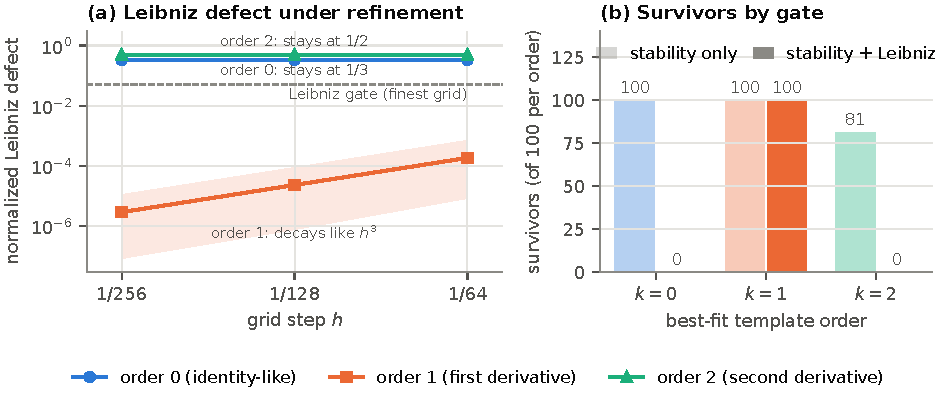
\includegraphics[width=\linewidth]{fig_stencil_matched.pdf}
\caption{Matched stencil experiment. (a) Normalized Leibniz defect on three grids for the three declared orders (median, with the range over 100 candidates shaded). The defect of first-order stencils falls by roughly a factor of eight per halving of $h$, while identity-like and second-order stencils keep a defect that does not decay. (b) Survivors of each order under the stability gate alone (light) and with the Leibniz gate added (solid). Data in Table~\ref{tab:stencil-matched}.}
\label{fig:stencil}
\end{figure}

The mechanism is visible in the limiting defects, independent of any fit.
For an identity-like operator the product-rule residual tends to $fg-fg-fg=-fg$, whose normalized size is about $1/3$.
For a second-derivative operator it tends to $(fg)''-f''g-fg''=2f'g'$, which on the pair $(x,x^2)$ gives exactly $1/2$ before the $10^{-12}$ denominator regularization.
For a first-derivative operator the residual tends to zero, and with $M_2=M_3=0$ it decays like $h^3$.
The Leibniz gate therefore discriminates between orders for a reason that is a theorem, not a tuning artifact.

\paragraph{Why the population must be matched.}
A tempting but unmatched comparison would contrast two different populations.
In an unconstrained random population of $\StencilBaselineTotal$ stencils (half-widths $2$ and $3$), $\StencilBaselineSurvivors$ pass the stability gate and all of them fit order~$0$, as expected, because a generic stencil acts to leading order as multiplication by $\sum_jc_j$.
In a population first projected onto the first-derivative moment conditions ($M_0=0$, $M_1=1$, and $M_2,M_3$ near zero), every one of the $\StencilLegacyTested$ candidates tested already fits order~$1$ before any gate, and the stability gate alone keeps the same $\StencilLegacySurvivors$ survivors as the stability and Leibniz gates together.
Comparing these two populations would credit the Leibniz gate with a selection that the moment normalization had already made.
The matched design holds the population fixed and varies only the gate.

\paragraph{A sampled search for false positives.}
We also searched for stencils that pass a Leibniz gate yet do not resemble any of $f$, $f'$, $f''$.
This search uses a different, pointwise defect: for $L_hf=h^{-1}\sum_jc_jf(\cdot+jh)$, the maximum over interior points and over the three pairs $(x,x^2)$, $(\sin 2\pi x,e^x)$, $(x^2,e^x)$ of
\[
  \frac{|L_h(fg)-(L_hf)g-f(L_hg)|}{|L_h(fg)|+10^{-12}},
\]
A candidate passes if the $\ell^2$ norm of its $h^{-1}$-scaled finest-grid output exceeds $10^{-6}$ for at least one test function and the three values $\Def_0,\Def_1,\Def_2$ of this defect satisfy $\Def_2<\text{threshold}$, $\Def_2<\text{ratio}\cdot\Def_1$, and $\Def_1<\text{ratio}\cdot\Def_0$; no stability gate is applied.
Among $\StencilHuntTested$ candidates ($\StencilHuntPerMode$ unconstrained and $\StencilHuntPerMode$ normalized to $M_0=0$, $M_1=1$), none passed the gate at thresholds $(0.10,0.75)$ for $(\Def_2,\text{ratio})$, so the search relaxed them to $(0.20,0.85)$.
At the relaxed thresholds $\StencilHuntPassed$ candidates pass, all from the normalized population, and none has a best template-fit error above $\StencilHuntMinF$.
This is a sampled negative result.
It is not an exhaustive classification, and a three-grid stability test does not prove bounded operator norms on a function space.

\subsection{Integration as a packaged closure of sums}
\label{subsec:integration}
The same audit applies to sums.
On the grid $x_i=ih$ in $[0,1]$, consider the cumulative left rule $I_h(f)(x_i)=h\sum_{j<i}f_j$ and the cumulative trapezoid rule $T_h(f)(x_i)=h\sum_{j<i}(f_j+f_{j+1})/2$.
They satisfy exact discrete identities:
\[
  \delta_hI_h(f)(x_i)=f_i,\qquad
  \delta_hT_h(f)(x_i)=\tfrac12(f_i+f_{i+1}),\qquad
  T_h(f)(x_i)-I_h(f)(x_i)=\tfrac h2\,(f_i-f_0),
\]
and both are exactly additive over a split of the interval.
The left rule therefore satisfies a discrete fundamental theorem with zero defect, and its measured residual (about $\IntegrationFTLeftMax$ at most), like the additivity residuals (about $\IntegrationAddMax$ at most), is floating-point rounding.
We do not fit power laws to such residuals.

The informative diagnostics, maximized over the test family $\{\sin 2\pi x,\ e^x,\ 1,\ x,\ x^2\}$ on grids with $N\in\IntegrationNList$, are the following (Table~\ref{tab:integration}, Figure~\ref{fig:integration}).
\begin{itemize}
  \item \emph{Route mismatch.} The relative mismatch $\|I_h-T_h\|/(\|T_h\|+\varepsilon_0)$ falls to $\IntegrationRMAtSmallestH$ at the finest grid, with fitted slope $\IntegrationRMExponent$ in $h$. This matches the exact identity above: for a fixed nonzero antiderivative the relative mismatch is $O(h)$, since the grid-size factors of the two norms cancel.
  \item \emph{Trapezoid fundamental theorem.} For $f\in C^1$ with $\|f'\|_\infty\le M$, the pointwise defect $|\tfrac12(f_i+f_{i+1})-f_i|$ is at most $Mh/2$. In the unweighted $\ell^2$ norm over $N=1/h$ points this is $O(h^{1/2})$, and the fitted slope is $\IntegrationFTExponent$; in the $\sqrt h$-weighted norm, which approximates the $L^2$ norm, it is $O(h)$.
  \item \emph{Truth.} Agreement between two routes does not show that either computes an integral, so we also compare each rule with the exact antiderivative. The $\sqrt h$-weighted errors decrease to $\IntegrationLeftTruthFinest$ (left) and $\IntegrationTrapTruthFinest$ (trapezoid) at $N=1024$, consistent with the classical $O(h)$ and $O(h^2)$ error orders for $C^1$ and $C^2$ integrands.
\end{itemize}

% Auto-generated by scripts/export_results_tex.py from notes/math_review/
\begin{table}[htbp]
\centering
\caption{Integration diagnostics, each maximized over the test family. RM is the relative left/trapezoid route mismatch; $\mathrm{FT}_T$ is the trapezoid fundamental-theorem defect in the raw and $\sqrt h$-weighted $\ell^2$ norms; the last two columns are $\sqrt h$-weighted errors against the exact antiderivative.}
\label{tab:integration}
\small
\begin{tabular}{rrrrrr}
\toprule
$N$ & RM & $\mathrm{FT}_T$ raw & $\mathrm{FT}_T$ weighted & Left error & Trapezoid error \\
\midrule
128 & $0.0142$ & $0.196$ & $0.0174$ & $3.42\times 10^{-3}$ & $3.91\times 10^{-5}$ \\
256 & $7.09\times 10^{-3}$ & $0.139$ & $8.68\times 10^{-3}$ & $1.71\times 10^{-3}$ & $9.79\times 10^{-6}$ \\
512 & $3.54\times 10^{-3}$ & $0.0982$ & $4.34\times 10^{-3}$ & $8.52\times 10^{-4}$ & $2.45\times 10^{-6}$ \\
1024 & $1.77\times 10^{-3}$ & $0.0694$ & $2.17\times 10^{-3}$ & $4.25\times 10^{-4}$ & $6.12\times 10^{-7}$ \\
\bottomrule
\end{tabular}
\end{table}


\begin{figure}[htbp]
\centering
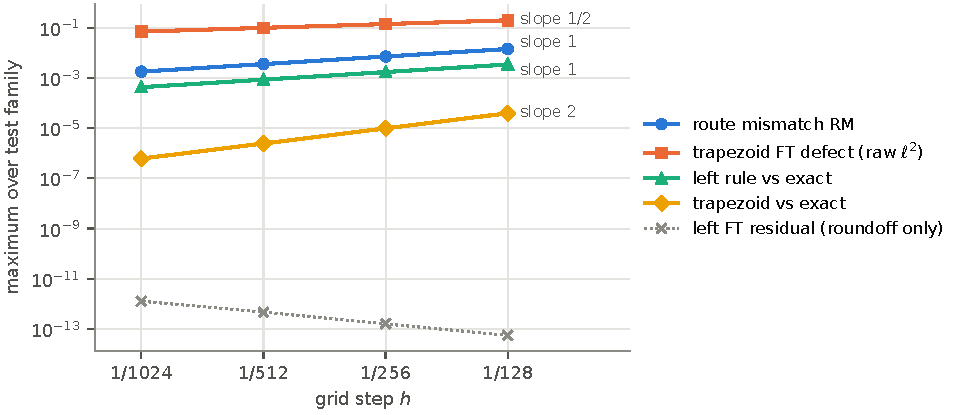
\includegraphics[width=0.92\linewidth]{fig_integration.pdf}
\caption{Integration diagnostics under refinement (log--log). Annotated slopes are the theoretical orders. The left-rule fundamental-theorem residual (grey) is rounding error around an exact identity and is shown only for contrast. Data in Table~\ref{tab:integration}.}
\label{fig:integration}
\end{figure}

\section{Route dependence under a change of coordinates}
\label{sec:exhibit-holonomy}

This exhibit makes the protocol role (\Pthree) quantitative.
When there are two natural routes from staged data to a packaged object, the routes need not agree at finite resolution.
Their disagreement is a defect, and a stable closure should make it shrink under refinement.

\subsection{Two routes to one derivative}
Let $g(y)=\sin(2\pi y)+0.1\cos(6\pi y)+e^{-y}$ and consider the change of coordinates
\[
  y=\varphi(x)=x+\varepsilon x^2,\qquad x\in[0,1],\quad\varepsilon=\HolonomyEps .
\]
The map is a valid chart, with $\varphi'>0$ on $[0,1]$, whenever $\varepsilon>-1/2$.
Both routes below estimate the same quantity, $g'(\varphi(x))$, at the same interior points $x$ of a grid with step $h$:
\begin{enumerate}
  \item \emph{Route A (differentiate in the target, then pull back).} Sample $g$ on a uniform $y$-grid with step $h$ that covers the whole image $\varphi([0,1])$, refine it to step $h/2$ by linear interpolation, take central differences, and interpolate the result at the points $\varphi(x)$.
  \item \emph{Route B (pull back, then differentiate in the source).} Interpolate the same samples to obtain $g\circ\varphi$ on the $x$-grid, refine to step $h/2$, take central differences in $x$, divide by $\varphi'(x)$ (the chain rule), and interpolate back to the evaluation points.
\end{enumerate}
At finite $h$ the two routes differ because interpolation, refinement, and differencing do not commute.

\subsection{Diagnostic}
We measure the relative route mismatch~\eqref{eq:rm-generic},
\begin{equation}\label{eq:rm-def}
  \RM(h)\;=\;\frac{\|R_A(h)-R_B(h)\|_2}{\|R_A(h)\|_2+\varepsilon_0},\qquad \varepsilon_0=10^{-12},
\end{equation}
over the common evaluation points, on grids with $N=1/h\in\HolonomyNList$.
Two controls accompany it.
With the identity chart ($\varepsilon=0$) the routes coincide exactly, and the measured mismatch is $\HolonomyNullRMMax$ on every grid, which confirms that the comparison is aligned.
And because mutual agreement does not show that either route is correct, we also measure each route's RMS error against the exact value $g'(\varphi(x))$.

\subsection{Results}
The mismatch decreases monotonically, from $4.76\times 10^{-3}$ at $N=64$ to $\HolonomyRMFinest$ at $N=512$ (Table~\ref{tab:holonomy}, Figure~\ref{fig:holonomy}).
A least-squares fit of $\log\RM$ against $\log h$ over the four grids gives slope $p=\HolonomyExponent$ with $R^2=\HolonomyFitRtwo$.
Both routes also converge to the exact derivative.

% Auto-generated by scripts/export_results_tex.py from notes/math_review/
\begin{table}[htbp]
\centering
\caption{Coordinate-change diagnostic: relative route mismatch and the RMS error of each route against the exact derivative $g'(\varphi(x))$.}
\label{tab:holonomy}
\small
\begin{tabular}{rrrrr}
\toprule
$N$ & $h$ & $\mathrm{RM}(h)$ & Route A error & Route B error \\
\midrule
64 & $0.0156$ & $4.76\times 10^{-3}$ & $0.0140$ & $0.0329$ \\
128 & $7.81\times 10^{-3}$ & $1.32\times 10^{-3}$ & $4.12\times 10^{-3}$ & $9.22\times 10^{-3}$ \\
256 & $3.91\times 10^{-3}$ & $4.91\times 10^{-4}$ & $1.00\times 10^{-3}$ & $2.83\times 10^{-3}$ \\
512 & $1.95\times 10^{-3}$ & $2.25\times 10^{-4}$ & $2.47\times 10^{-4}$ & $1.13\times 10^{-3}$ \\
\bottomrule
\end{tabular}
\end{table}


\begin{figure}[htbp]
\centering
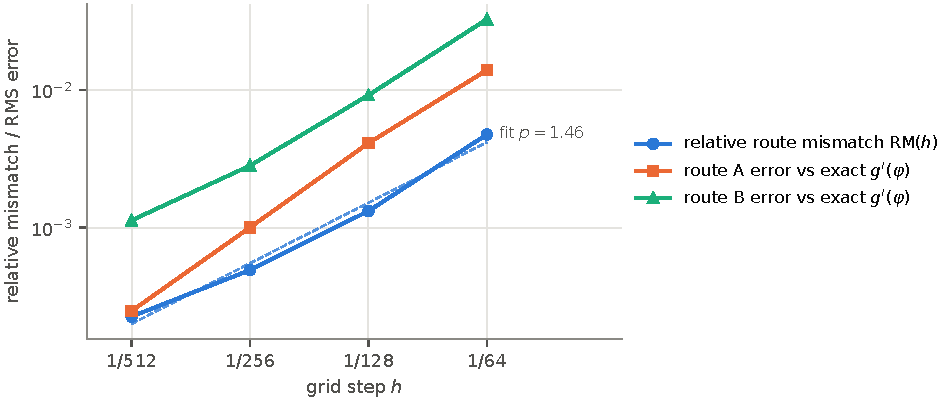
\includegraphics[width=0.92\linewidth]{fig_holonomy.pdf}
\caption{Coordinate-change diagnostic (log--log). The relative mismatch between the two routes (circles; dashed line, least-squares fit) decreases under refinement, and each route approaches the exact derivative $g'(\varphi(x))$. The identity chart gives zero mismatch on every grid and is not shown on the logarithmic axis. Data in Table~\ref{tab:holonomy}.}
\label{fig:holonomy}
\end{figure}

\subsection{Interpretation}
The fitted exponent is a four-point summary of a finite-grid trend, not an asymptotic convergence order.
For a smooth $g$, piecewise-linear interpolation already guarantees a first-order error bound away from the boundary; the observed decay is faster than that on these grids, but nothing here establishes a universal rate.
Nor does the zero mismatch of the identity chart prove that every effect of nonlinear interpolation has been removed: route dependence is precisely what is being measured.

What the exhibit does establish is the shape of a \Pthree\ audit.
Two admissible routes are made to estimate the same quantity at the same points, a null control calibrates the comparison, a truth check guards against two routes agreeing on a wrong answer, and the mismatch is tracked under refinement.
In differential geometry, genuine holonomy is tied to curvature and to obstructions to patching local descriptions; nothing of that kind is claimed here.
A decaying route mismatch says only that, for this staged protocol, the two routes become compatible as resolution increases.
It implies no direction of time and no irreversible ordering of states.

\section{Prime closures: a control regime and a failure regime}
\label{sec:exhibit-prime}

This exhibit applies the closure audit to a classic compression of discrete structure into an analytic object: the integers and the primes into the zeta function.
The aim is not to prove anything about $\zeta$.
It is to show that the same route-mismatch machinery used for derivatives separates a regime where two staged descriptions provably converge to a common object from a regime where naive staging fails.

\subsection{Two staged descriptions}
For $\Re(s)>1$ the zeta function has an additive and a multiplicative description,
\[
  \zeta(s)=\sum_{n\ge 1}n^{-s}=\prod_p\frac{1}{1-p^{-s}},
\]
see, for example, \cite{Titchmarsh1986}.
We stage both at a cutoff $N$ with the smoothing weight $w(u)=e^{-u}$:
\begin{align*}
  S_N(s)&:=\sum_{n=1}^{N}w(n/N)\,n^{-s},\\
  P_N(s)&:=\exp\Bigl(\sum_{p\le N}w(p/N)\,\bigl(-\log(1-p^{-s})\bigr)\Bigr)=\prod_{p\le N}(1-p^{-s})^{-w(p/N)}.
\end{align*}
The Euler-side weights act on the logarithms of the factors, and $w\equiv 1$ would give the sharp partial sum and partial product.
In the language of Section~\ref{sec:dictionary}, $S_N$ is an additive staging protocol and $P_N$ a multiplicative one; a stable closure requires them to become compatible as $N$ grows.

\subsection{Packaging maps}
To compare staged functions across regions we apply three simple packaging maps.
With the completion factor $C(s)=\tfrac12 s(s-1)\pi^{-s/2}\Gamma(s/2)$, set
\begin{align*}
  \mathrm{Raw}(F)&=F, \qquad \mathrm{Comp}(F)(s)=C(s)F(s),\\
  \mathrm{Sym}(F)(s)&=\tfrac12\bigl(\mathrm{Comp}(F)(s)+\mathrm{Comp}(F)(1-s)\bigr).
\end{align*}
$\mathrm{Comp}$ is a one-sided completion and $\mathrm{Sym}$ enforces the symmetry $s\leftrightarrow 1-s$ by construction.
Neither is an analytic continuation scheme.
In the convergence region we use $\mathrm{Comp}$, because $\mathrm{Sym}$ would evaluate the truncations at $1-s$ with $\Re(1-s)<0$, far outside their domain of validity; in the critical strip we use $\mathrm{Sym}$ as a prototype of self-dual packaging.
The two regimes thus differ in both the region and the packaging map: the exhibit compares two staging--packaging pairs, not a single isolated variable.

\subsection{Diagnostics}
Let $\mathrm{Pack}$ be the packaging map of a regime, $A_N=\mathrm{Pack}(S_N)$ and $B_N=\mathrm{Pack}(P_N)$, and let $K$ be a finite test set: $\sigma\in\PrimeSigmaConvList$ in the convergence region or $\sigma\in\PrimeSigmaStripList$ in the strip, with $t\in\PrimeTList$ and $s=\sigma+it$.
With cutoffs $N\in\PrimeNList$ we compute the route mismatch
\[
  \RM_2(N)=\frac{\bigl(\sum_{s\in K}|A_N(s)-B_N(s)|^2\bigr)^{1/2}}{\bigl(\sum_{s\in K}|A_N(s)|^2\bigr)^{1/2}+\varepsilon_0}
\]
with $\varepsilon_0=10^{-30}$ (and its analogue $\RM_\infty$ with maximum norms), together with two error ledgers against a reference computed by \texttt{mpmath.zeta} under the same packaging,
\[
  \mathrm{Err}_S(N)=\frac{\|A_N-\mathrm{Pack}(\zeta)\|_2}{\|\mathrm{Pack}(\zeta)\|_2+\varepsilon_0},\qquad
  \mathrm{Err}_P(N)=\frac{\|B_N-\mathrm{Pack}(\zeta)\|_2}{\|\mathrm{Pack}(\zeta)\|_2+\varepsilon_0}.
\]
All arithmetic, including the ratios $n/N$ and $p/N$ inside the smoothing weights, is carried out at $\PrimeDPS$-digit working precision in \texttt{mpmath}; the reported summaries are stored as double-precision numbers.
In the convergence region the error ledgers are accuracy tests; in the strip they measure how far naive staging is from the analytically continued function.

\subsection{The control regime is provably convergent}
In the region $\Re(s)>1$ the finite trend has a proof behind it.

\begin{proposition}[Convergence of the staged closures]\label{prop:prime-control}
Let $K$ be a compact subset of $\{\Re(s)>1\}$. Then $S_N\to\zeta$ and $P_N\to\zeta$ uniformly on $K$ as $N\to\infty$, and the same holds after applying $\mathrm{Comp}$. Consequently $\RM_2(N)$, $\mathrm{Err}_S(N)$, and $\mathrm{Err}_P(N)$ tend to zero on every finite $K$ in this region.
\end{proposition}

\begin{proof}
Let $\sigma_0>1$ be the minimum of $\Re(s)$ on $K$. Then $|n^{-s}|\le n^{-\sigma_0}$, which is summable, while the weights $w(n/N)$ lie in $[0,1]$ and tend to $1$ for each fixed $n$; dominated convergence, applied uniformly in $s\in K$, gives $S_N\to\zeta$ uniformly. For primes $|p^{-s}|\le p^{-\sigma_0}\le 2^{-\sigma_0}<1$, so the principal logarithm is given by its power series and $|{-\log(1-p^{-s})}|\le p^{-\sigma_0}/(1-2^{-\sigma_0})$, again summable. The weighted log-sums therefore converge uniformly to $\sum_p-\log(1-p^{-s})$, and continuity of $\exp$ on the bounded range gives $P_N\to\zeta$ by the Euler product. The factor $C(s)$ is analytic, hence bounded, on $K$, so multiplication by it preserves uniform convergence. The numerators of the three diagnostics therefore tend to zero, and their denominators are bounded below by $\varepsilon_0>0$.
\end{proof}

\subsection{Results}
Table~\ref{tab:prime-rm} and Figure~\ref{fig:prime-rm} report both regimes.
In the convergence region all three diagnostics decrease with $N$; the route mismatch reaches $\RM_2(800)=\PrimeRMConvAtEightHundred$.
In the strip they behave very differently: $\RM_2$ grows from $\PrimeRMStripAtFifty$ at $N=50$ to $\PrimeRMStripAtEightHundred$ at $N=800$, the Euler-side error reaches $\PrimeErrPStripAtEightHundred$, and even the additive error grows to $\PrimeErrSStripAtEightHundred$.

% Auto-generated by scripts/export_results_tex.py from notes/math_review/
\begin{table}[htbp]
\centering
\caption{Prime closure diagnostics. Left: convergence region with one-sided completion. Right: critical strip with symmetrized completion.}
\label{tab:prime-rm}
\small
\begin{tabular}{r rrr rrr}
\toprule
& \multicolumn{3}{c}{$\Re(s)\in\PrimeSigmaConvList$} & \multicolumn{3}{c}{$\Re(s)\in\PrimeSigmaStripList$} \\
\cmidrule(lr){2-4}\cmidrule(lr){5-7}
$N$ & $\mathrm{RM}_2$ & $\mathrm{Err}_S$ & $\mathrm{Err}_P$ & $\mathrm{RM}_2$ & $\mathrm{Err}_S$ & $\mathrm{Err}_P$ \\
\midrule
50 & $0.0760$ & $0.209$ & $0.147$ & $340$ & $6.59$ & $2.12\times 10^{3}$ \\
100 & $0.0698$ & $0.172$ & $0.112$ & $6.00\times 10^{3}$ & $10.4$ & $6.03\times 10^{4}$ \\
200 & $0.0667$ & $0.142$ & $0.0848$ & $6.20\times 10^{5}$ & $16.5$ & $9.85\times 10^{6}$ \\
400 & $0.0613$ & $0.118$ & $0.0654$ & $3.14\times 10^{8}$ & $27.1$ & $8.29\times 10^{9}$ \\
800 & $0.0524$ & $0.0985$ & $0.0506$ & $5.01\times 10^{12}$ & $43.7$ & $2.17\times 10^{14}$ \\
\bottomrule
\end{tabular}
\end{table}


\begin{figure}[htbp]
\centering
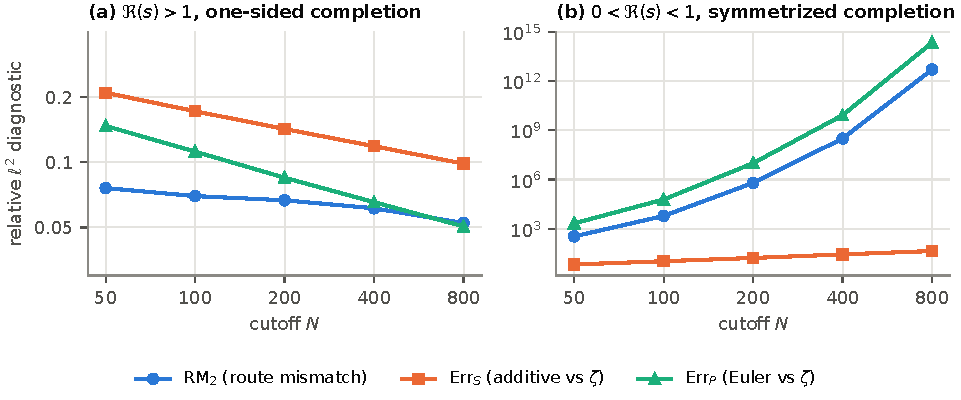
\includegraphics[width=\linewidth]{fig_prime.pdf}
\caption{Prime closure diagnostics. (a) For $\Re(s)>1$, with one-sided completion, the route mismatch and both errors against $\zeta$ decrease over the tested cutoffs, consistent with the convergence to zero established by Proposition~\ref{prop:prime-control}. (b) In the critical strip, with symmetrized completion, the same naive protocols drift apart by many orders of magnitude. The vertical scales differ by design; data in Table~\ref{tab:prime-rm}.}
\label{fig:prime-rm}
\end{figure}

To check that the stored summaries are not artifacts of the working precision, the full grid was recomputed independently at $\PrimeCheckDPS$ digits.
Every reported value of $\RM_2$, $\RM_\infty$, $\mathrm{Err}_S$, and $\mathrm{Err}_P$ agrees with the $\PrimeDPS$-digit computation to double precision.
This is a stability check of double-precision summaries, not an interval certificate.

\subsection{Interpretation}
The growth in the strip has an ordinary explanation.
For real $s\in(0,1)$ the smoothed additive sums grow like $N^{1-s}$, and the weighted prime sums $\sum_{p\le N}w(p/N)\,p^{-s}$ diverge; since $-\log(1-p^{-s})\ge p^{-s}$, they are lower bounds for the logarithmic Euler sums, which therefore diverge as well.
Applying a completion factor or a symmetry projection does not repair truncation formulas that are invalid in the region.
The measurement is therefore a finite record of a feasibility failure of these staging--packaging pairs on this grid.
It is not a theorem that the mismatch blows up at every point of the strip, and it carries no information about the location of the zeros of $\zeta$.

The methodological point is that the same route-mismatch audit used for derivatives separates the two regimes, and that in the regime where it reports success there is a short proof that success is correct.
A staging scheme that is valid in the strip, such as one built on the approximate functional equation, is the natural next protocol to audit with the same tools (Section~\ref{sec:discussion}).

\section{A positivity toy: interaction signs and zero confinement}
\label{sec:exhibit-passivity}

A recurring motif in the framework is that the most rigidifying feasibility conditions are positivity conditions.
In physics, passivity constraints strongly restrict the analytic structure of response functions \cite{Willems1972II}; in mathematics, stability requirements often take the form of nonnegative quadratic forms, positive-definite kernels, or sign conditions on coefficients.
This exhibit gives a small, exactly understood instance: as a sign constraint on interactions is tightened, the zeros of a partition polynomial move onto a symmetry locus.

\subsection{The polynomial and its symmetries}
Take $n=\PassivityN$ spins $\sigma_i\in\{-1,1\}$ on a cycle with edge couplings $J_e$ and inverse temperature $\beta=\PassivityBeta$, and let
\[
  Z(z)\;=\;\sum_{\sigma\in\{-1,1\}^n}\exp\Bigl(\beta\sum_{e=\{i,j\}}J_e\,\sigma_i\sigma_j\Bigr)\,z^{\#\{i:\ \sigma_i=-1\}}\;=\;\sum_{k=0}^{n}a_k z^k,
\]
computed by direct enumeration.
Every coefficient $a_k$ is positive, whatever the signs of the $J_e$.
Reversing all spins leaves the interaction energy unchanged and exchanges $k$ with $n-k$, so $a_k=a_{n-k}$: the polynomial is palindromic as a matter of mathematics.
(The computation symmetrizes the coefficients numerically, which only removes floating-point summation asymmetry.)

A real palindromic polynomial has its roots closed under $z\mapsto 1/z$ and under complex conjugation, hence under the combined anti-involution $z\mapsto 1/\bar z$.
The fixed-point set of that anti-involution is the unit circle $|z|=1$, which is the natural symmetry locus.
(The inversion $z\mapsto 1/z$ alone fixes only $\pm 1$.)
Neither symmetry forces the roots onto the circle, and neither does positivity of the coefficients: $1+3z+z^2$ is real, palindromic, and positive, yet its two roots are real, negative, and off the circle.

\subsection{The feasibility parameter}
The couplings are drawn independently from a normal distribution with mean $0$ and standard deviation $\PassivityJScale$ (seed $0$), so they have mixed signs.
We tighten their signs with the clipped family
\[
  J_e(\lambda)=\max(J_e,0)+\lambda\min(J_e,0),\qquad\lambda\in[0,1],
\]
so that $\lambda=1$ is the original mixed-sign system and $\lambda=0$ removes every negative interaction.
This is an interaction-sign constraint; it is not a frequency-domain passivity condition, and we use ``positivity'' in that narrow sense.

At the endpoint the zeros are located by a classical theorem.
For $\beta\ge 0$ all effective couplings $\beta J_e(0)$ are nonnegative, and the Lee--Yang circle theorem \cite{LeeYang1952} applies to this finite ferromagnetic Ising polynomial, including zero couplings and disconnected components: every zero of $Z_0$ lies on $|z|=1$.
This is an imported theorem, not a numerical discovery.

A two-spin system shows the mechanism in closed form.
With one edge and $K=\beta J$, the polynomial is, up to a positive factor,
\[
  z^2+2e^{-2K}z+1 .
\]
If $K\ge 0$ the middle coefficient lies in $(0,2]$, the roots are complex conjugates with product $1$, and both lie on the unit circle.
If $K<0$ the middle coefficient exceeds $2$, and the roots are two negative reals with product $1$, one inside and one outside the circle.
Shrinking a negative coupling toward zero moves the coefficient toward $2$ and the roots toward $-1$.
This exact example supplies the motif that tightening the sign constraint \emph{can} confine zeros; no monotonicity theorem for arbitrary graphs is claimed.

\subsection{Measurement}
We compute all zeros of $Z_\lambda$ and measure their radial deviations $d_i=\bigl||z_i|-1\bigr|$, summarized by $\mathrm{mean\_dev}(\lambda)=\frac1n\sum_id_i$ and $\mathrm{max\_dev}(\lambda)=\max_id_i$.
The computation respects the structure of the problem.
Partition functions of disjoint subsystems multiply, so we factor $Z_\lambda$ over the connected components of the graph of nonzero couplings, with edges removed only when a coupling is exactly zero, and find the roots of each factor separately.
An isolated spin contributes exactly $1+z$.
Every component factor is palindromic, and a palindromic polynomial of odd degree has $-1$ as a root.
At $\lambda=0$ the components have degrees $\PassivityComponentsLamZero$, so $z=-1$ is a root of multiplicity four: one from each of the two cubic factors and one from each of the two isolated spins.
Finding the roots of the full degree-$12$ polynomial instead would split that fourfold root numerically and report spurious deviations of order $10^{-4}$; a small backward residual of the computed roots does not control the forward position of a repeated root.

\subsection{Results}
Table~\ref{tab:passivity} and Figure~\ref{fig:passivity-toy} show the outcome.
The mean deviation decreases at every sampled step, from $\PassivityMeanDevLamOne$ at $\lambda=1$ (where the largest deviation is $\PassivityMaxDevLamOne$) to $\PassivityMeanDevLamZero$ at $\lambda=0$, which is floating-point rounding: at the endpoint every zero is on the circle, as the Lee--Yang theorem requires.
As an independent check, the zeros at $\lambda=1$ and $\lambda=0$ were recomputed at $\PassivityCheckDPS$ digits with a separate enumeration and component decomposition.
The largest distance between matched roots is $\PassivityMatchLamOne$ at $\lambda=1$ and $\PassivityMatchLamZero$ at $\lambda=0$.
This high-precision computation is a consistency check, not an interval certificate; the endpoint statement rests on the theorem.

% Auto-generated by scripts/export_results_tex.py from notes/math_review/
\begin{table}[htbp]
\centering
\caption{Positivity toy: radial deviation of the zeros from the unit circle. The second column lists the degrees of the component factors of $Z_\lambda$; at $\lambda=0$ the deviations are at floating-point roundoff.}
\label{tab:passivity}
\small
\begin{tabular}{rlrr}
\toprule
$\lambda$ & Component degrees & mean\_dev & max\_dev \\
\midrule
$1$ & 12 & $0.872$ & $7.11$ \\
$0.7$ & 12 & $0.580$ & $4.27$ \\
$0.4$ & 12 & $0.350$ & $2.27$ \\
$0.2$ & 12 & $0.201$ & $1.22$ \\
$0.1$ & 12 & $0.0947$ & $0.718$ \\
$0$ & 3,3,4,1,1 & $1.55\times 10^{-15}$ & $6.00\times 10^{-15}$ \\
\bottomrule
\end{tabular}
\end{table}


\begin{figure}[htbp]
\centering
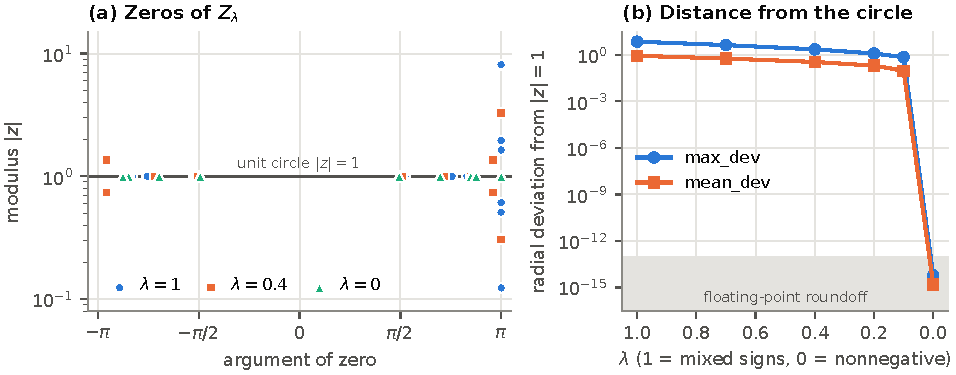
\includegraphics[width=\linewidth]{fig_passivity.pdf}
\caption{Positivity toy. (a) Zeros of $Z_\lambda$ plotted by argument and modulus, so that the unit circle is the horizontal line $|z|=1$; reciprocal pairs appear symmetric about it on the logarithmic scale. With mixed-sign couplings ($\lambda=1$) several zeros lie on the negative real axis (argument $\pi$) far from the circle; with nonnegative couplings ($\lambda=0$) all lie on it. (b) Mean and maximum radial deviation as the negative couplings are scaled to zero; the endpoint is at rounding level. Data in Table~\ref{tab:passivity}.}
\label{fig:passivity-toy}
\end{figure}

\subsection{Interpretation}
The endpoint is a theorem and the decrease across the five sampled steps in $\lambda$ is a finite observation for one sampled system.
The exhibit's role in this paper is to show a recognizable pattern under explicit control: a symmetry (\Ptwo) singles out a locus, a sign constraint acts as the feasibility condition, and the radial deviations of the zeros serve as the ledger (\Psix).
It suggests why problems of confining zeros to a self-dual locus invite positivity formulations, and it complements the prime exhibit, where staging and symmetrization without any additional feasibility condition did not yield a stable closure.
It establishes nothing about $\zeta$.

\section{Reproducibility}
\label{sec:reproducibility}

The tables, the data figures, and the numerical values that the text imports as macros are generated by scripts from commit-visible artifacts in the companion repository.
The few numbers quoted literally in the abstract and in running prose were checked against the same artifacts; the closure-engine diagram (Figure~\ref{fig:engine}) is drawn directly in \TeX.

\subsection{Regenerating the results}
From the repository root, one command reruns the full mathematical pipeline:
\begin{verbatim}
bash scripts/check_all.sh --math-only
\end{verbatim}
It runs the Python regression tests ($\PythonTestsPassed$ tests), builds the Lean project, prints the axioms of every exported Lean declaration and rejects any axiom outside the standard three (Appendix~\ref{app:formal}), reruns every experiment at its default settings (including the matched stencil control and the false-positive search), repeats the prime and Ising computations at higher precision, and audits the resulting artifacts.
The outputs are written to \path{notes/math_review/}; the file \path{verification.json} there records the final results, the package versions, and SHA-256 hashes of the source files.
All randomized experiments use fixed seeds; the remaining computations are deterministic.

The paper is then rebuilt from those artifacts:
\begin{verbatim}
python scripts/export_results_tex.py
python scripts/make_paper_figures.py
bash scripts/build_math_paper.sh
\end{verbatim}
The first script writes the numerical macros and tables in \path{tex/math_instantiation/generated/}; the second draws every data figure into \path{figures/paper/}; the third compiles the PDF.

\subsection{Environment}
The recorded runs used Python 3.12.3 with NumPy 2.5.3, SciPy 1.18.1, mpmath 1.3.0, and Matplotlib 3.11.2.
The Lean project pins the toolchain label \texttt{v4.9.1} (which reports Lean version 4.9.0) and mathlib commit \texttt{09d33efc68d3ad52db77b731d7253675395a14aa}; imports are restricted to the modules actually used.

\subsection{What the artifact contract guarantees}
\begin{remark}[Artifact contract]
Every numerical value in the generated tables and in the macros imported from \path{generated/macros.tex}, and every plotted point in Figures~\ref{fig:stencil}--\ref{fig:passivity-toy}, is read from the JSON artifacts in \path{notes/math_review/} by \path{scripts/export_results_tex.py} or \path{scripts/make_paper_figures.py}.
A reported number therefore means ``the value recorded in the committed artifact when the PDF was built''.
\end{remark}

Consistency between the paper and the repository holds when the generated files are regenerated and the PDF is rebuilt from the same artifact snapshot; the mathematical pipeline alone does not touch the paper, and the \TeX\ build does not regenerate or verify the generated files.
The contract does not guarantee bit-identical results across platforms, and the numerical results remain diagnostics: none of them is an interval-arithmetic or exhaustive proof.

\section{Discussion}
\label{sec:discussion}

\subsection{What is established}
The paper offers three things.
First, a vocabulary for treating mathematical constructions as closures (Sections~\ref{sec:dictionary} and~\ref{sec:packaging-engine}), with the two contracts that make the vocabulary precise: packaging needs a genuine pseudometric, and an operator becomes a packaged law only if it respects the packaging.
Second, machine-checked anchors that pin the calculus exhibit to exact statements: the finite-difference product rule, the limit bridge to the Leibniz rule, the classification of polynomial derivations, and the packaging, descent, and linear route bounds.
Third, numerical diagnostics that were able to fail, together with the controls that make their outcomes interpretable: a matched population for the stencil experiment, null charts and truth checks for the route comparisons, a proof for the prime control regime, and a classical theorem for the endpoint of the positivity toy.

\subsection{Limits of the claims}
\paragraph{Diagnostics are not theorems.}
The stencil experiment shows that, in a fixed population of $\StencilMatchedTotal$ normalized stencils, the Leibniz gate keeps exactly the first-derivative ones, and it explains why through the limiting defects.
It is not a classification of all local operators, and the false-positive search is sampled, not exhaustive.
Fitted exponents, such as $p\approx\HolonomyExponent$ for the coordinate change, summarize a few grids and are not asymptotic orders.

\paragraph{Prime closures are a baseline, not a continuation.}
In the region $\Re(s)>1$ the diagnostics confirm what Proposition~\ref{prop:prime-control} proves.
In the strip they document that naive staging fails, for reasons that are already classical, and they say nothing about the zeros of $\zeta$.

\paragraph{The positivity toy is a motif.}
Its endpoint is the Lee--Yang theorem; its intermediate trend is one sampled system.
The sign constraint it uses is not a general passivity condition.

\paragraph{The dictionary is adopted.}
The six roles organize constructions that are already present in mathematical practice.
They do not supply the comparison spaces, Cauchy conditions, or descent estimates; those must be proved in each case, as Sections~\ref{sec:packaging-engine} and~\ref{sec:exhibit-calculus} do for the calculus exhibit.

\subsection{Next steps}
\paragraph{Analytic closure.}
The calculus exhibit could replace its finite gates with classical consistency and stability hypotheses, and state the regularity classes under which each ledger term vanishes.
The coordinate-change exhibit could connect its observed decay to truncation-order estimates for the interpolation and differencing steps.

\paragraph{Prime ledgers that are valid in the strip.}
A natural next protocol uses the approximate functional equation as an additive staging that is valid in the critical strip, compared against smoothed prime-sum or logarithmic-derivative ledgers in regimes where they are controlled \cite{Titchmarsh1986}.
The present exhibit is the baseline against which such a scheme would be measured.

\paragraph{Formalization.}
The quotient-valued derivation of Proposition~\ref{prop:quotient-derivation} and the convergence argument of Proposition~\ref{prop:prime-control} are short and standard, and both are natural candidates for mechanization alongside the existing bridges.

\subsection{Why the closure lens helps}
Even at this modest scale, the closure lens separates two questions that are easy to conflate: whether a formula for a limit object exists, and whether the staged protocol behind it is stable under refinement and compatible with the operations one wants to perform on it.
The same ledger, packaging, and route-mismatch ideas apply to measure and integration, to limits in functional analysis, to the patching of local descriptions in geometry, and to spectral constructions.

\subsection{Closing}
The slogan ``to count a stone with six birds'' is meant literally.
Counting is a staged discrete protocol; calculus is a stable compression of that protocol under an accounting ledger; and higher layers arise by repeating the packaging with new constraints and new mismatch diagnostics.
The aim of the paper is to make those roles explicit, auditable, and reusable.


\section*{Data availability}
All code, data, Lean sources, and reproducibility artifacts are available in the companion repository at \url{https://github.com/ioannist/six-birds-mathematics}.

\section*{Acknowledgments}
The author acknowledges the use of Lean~4, mathlib, and standard Python scientific libraries (NumPy, mpmath, Matplotlib).

\section*{Funding and conflicts of interest}
This research received no external funding. The author declares no conflicts of interest.

\bibliographystyle{plainnat}
\bibliography{bib/refs}

\appendix
\section{Formal anchors in Lean}
\label{app:formal}

Table~\ref{tab:lean} lists the $\LeanExportCount$ declarations exported by \path{lean/Main.lean}.
For each, the review pipeline prints the transitive axioms with \texttt{\#print axioms} and checks that they are among \texttt{propext}, \texttt{Classical.choice}, and \texttt{Quot.sound}; no declaration depends on \texttt{sorryAx} or on a custom axiom.
The hypotheses visible in each statement are part of the claim: the limit bridge consumes convergence of the factor quotients, the packaging statement consumes a pseudometric, and the descent statement consumes a uniform Lipschitz bound.
None of the numerical experiments is formalized.

\begin{table}[htbp]
\caption{Exported Lean declarations and what they state. Files are under \texttt{lean/}.}
\label{tab:lean}
\small
\begin{tabularx}{\linewidth}{>{\raggedright\arraybackslash}p{0.42\linewidth}>{\raggedright\arraybackslash}X}
\toprule
Declaration & Statement \\
\midrule
\multicolumn{2}{l}{\emph{Finite differences} (\path{Diff/FiniteDifference.lean})} \\
\leanname{Diff.delta_mul_leibniz} & Over a field $F$ with $h\ne 0$: exact product rule with remainder (Lemma~\ref{lem:finite-diff-leibniz}). \\
\leanname{Diff.delta_add}, \leanname{Diff.delta_const_mul}, \leanname{Diff.delta_const} & $\delta_h$ is additive and homogeneous, and kills constants. \\
\leanname{Diff.tendsto_delta_mul} & Over $\mathbb R$: convergent factor quotients along a filter with $h_i\to 0$, $h_i\ne 0$ eventually, force the product quotient to converge to $a\,g(x)+f(x)\,b$. \\
\leanname{Diff.leibniz_of_tendsto_delta} & Along a nontrivial filter, any limit of the product quotient equals that value (Proposition~\ref{prop:limit-bridge}). \\
\midrule
\multicolumn{2}{l}{\emph{Polynomial derivations} (\path{Derivations/Polynomial.lean})} \\
\leanname{Derivations.derivation_ext_X} & For a commutative semiring $R$: two derivations of $R[X]$ agreeing on $X$ are equal. \\
\leanname{Derivations.polynomialDerivationEquiv} & $\mathrm{Der}_R(R[X],R[X])\simeq_R R[X]$, from mathlib's equivalence. \\
\leanname{Derivations.polynomialDerivationEquiv_apply_X}, \leanname{Derivations.polynomialDerivationEquiv_symm_apply_X} & The equivalence is evaluation at $X$, and its inverse sends $p$ to a derivation with value $p$ at $X$. \\
\leanname{Derivations.polynomialDerivationEquiv_symm_apply} & The inverse is $q\mapsto p\,q'$. \\
\leanname{Derivations.derivation_eq_derivative_of_X_eq_one} & $D(X)=1$ implies $D$ is the formal derivative (Theorem~\ref{thm:derivation-determined-by-X}). \\
\midrule
\multicolumn{2}{l}{\emph{Packaging, descent, and routes} (\path{Closure/})} \\
\leanname{Closure.vanishingDistSetoid} & Vanishing pseudometric distance between sequences is an equivalence relation (Proposition~\ref{prop:packaging}). \\
\leanname{Closure.stage_operator_respects_vanishing_dist} & Uniformly Lipschitz stage operators preserve it (Proposition~\ref{prop:descent}). \\
\leanname{Closure.route_gain_bound} & $\|C\|\le\|A\|\,\|B\|+\|C-A\circ B\|$ for continuous linear maps. \\
\leanname{Closure.idempotence_factorization}, \leanname{Closure.idempotence_defect_bound} & $L\circ L-L=L\circ(L-\mathrm{Id})$ and $\|L\circ L-L\|\le\|L\|\,\|L-\mathrm{Id}\|$ for a continuous linear $L$ (Proposition~\ref{prop:route-gain}). \\
\bottomrule
\end{tabularx}
\end{table}

\section{Version history}
\label{app:versions}

All versions on Zenodo share the concept DOI \href{https://doi.org/10.5281/zenodo.18402003}{10.5281/zenodo.18402003}.

\paragraph{Version 1 (28 January 2026).}
First release on Zenodo (DOI: \href{https://doi.org/10.5281/zenodo.18402004}{10.5281/zenodo.18402004}), with the dictionary, the closure engine, and four exhibits: stencil selection, coordinate-change route mismatch, prime closures, and the positivity toy.

\paragraph{Version 2 (February 2026).}
Added the integration exhibit and moved the manuscript to the MDPI preprint format. This version was not deposited on Zenodo.

\paragraph{Version 3 (4 October 2026).}
Zenodo DOI: \href{https://doi.org/10.5281/zenodo.23131954}{10.5281/zenodo.23131954}.
Followed a mathematical audit of the statements, code, and formalization.
\begin{itemize}
  \item The packaging and descent contracts are now explicit (Propositions~\ref{prop:packaging} and~\ref{prop:descent}), with the counterexamples that motivate them; the distinction between a quotient and a completion is stated.
  \item New Lean statements: linearity of $\delta_h$, the limit bridge to the Leibniz rule, the inverse formula for polynomial derivations, the packaging and descent contracts, and the linear route and idempotence bounds. The text now distinguishes convergence from boundedness (Example~\ref{ex:bounded-not-convergent}) and adds the quotient-valued derivation of Proposition~\ref{prop:quotient-derivation}.
  \item The stencil experiment was redesigned. In versions~1 and~2 the Leibniz-gated run selected candidates partly by their fitted order, which made the outcome ``all survivors are first order'' untestable, and it was compared with a stability-only run on a different population. The present matched experiment holds the population fixed, and fit labels never enter a gate.
  \item Integration: fitted power laws for residuals that are rounding error around exact identities were removed; raw and weighted norms are distinguished, and truth checks against exact antiderivatives were added.
  \item Coordinate change: the chart condition is enforced, the target grid covers the whole image, and route errors against the exact derivative are reported.
  \item Primes: the smoothing weights are now evaluated at full working precision; an $80$-digit recomputation and a convergence proof for the control regime (Proposition~\ref{prop:prime-control}) were added.
  \item Positivity toy: zeros are computed per connected component, which removes a spurious numerical splitting of the fourfold root at $z=-1$ (the endpoint deviation changes from about $3\times 10^{-4}$ to rounding level); the symmetry locus is identified as the fixed set of $z\mapsto 1/\bar z$; and the endpoint is identified as an instance of the Lee--Yang theorem.
  \item The abstract and text were rewritten for readability, the figures were redrawn from the audited artifacts, and the closure-engine diagram (Figure~\ref{fig:engine}) was added. The manuscript returns to a standard article layout. The title is unchanged.
\end{itemize}


\end{document}
